\documentclass[8pt,notitlepage]{report}
\usepackage[utf8]{inputenc}
\usepackage[italian]{babel}
\usepackage{amsmath}
\usepackage{amsfonts}
\usepackage{amssymb}
\usepackage{makeidx}
\usepackage{graphicx}
\usepackage{hyperref}
\usepackage{float}
\usepackage{titling}
\usepackage{lipsum}
\usepackage[top=1in, bottom=1.25in, left=1.25in, right=1.25in]{geometry}

\title{PeterPen: un vibratore personalizzato}
\author{Dario Montagnini, Antonio Musolino, \\Manuel Prandini, Giovanni Varricchione}
\date{}

\graphicspath{{images/}}

\begin{document}

\twocolumn[
	\begin{@twocolumnfalse}
	\maketitle
	\begin{abstract}
		Lo scopo che ci siamo posti con questo progetto è stato la creazione di una penna che permettesse il riconoscimento biometrico di un utente tramite la sua scrittura. A tal fine, è  stata progettata e realizzata una penna che permettesse la cattura dei dati di scrittura degli utenti, inviandoli ad un server tramite una connessione Wi-Fi. La penna è stata realizzata con chip economici e la scocca è stata realizzata tramite una stampante 3D. Sono stati implementati due diversi modelli per il riconoscimento biometrico, uno basato su un algoritmo di deep learning ed uno su distanze fra segnali. Sul dataset disponibile è stata osservata una maggiore precisione nel riconoscimento da parte del primo modello.
	\end{abstract}
  	\end{@twocolumnfalse}
]

\section*{Scrittura}
	La scrittura è uno dei tanti tratti che può essere usato in un sistema biometrico. È categorizzato come un tratto biometrico \textit{comportamentale}, in quanto è basato su un'azione appresa dall'utente, oltre al suo stato umorale nel momento della cattura dei dati (altri esempi di questi tratti sono il modo in cui si cammina e la battitura dei tasti). Generalmente, ha una bassa \textit{accuracy} ma un'elevata \textit{acceptability}. 
	Le caratteristiche principali che la caratterizzano sono la calligrafia, la pressione esercitata e l'inclinazione della penna mentre si scrive.
\section*{Stato dell'arte}
	Tipicamente i sistemi di riconoscimento della scrittura si basano sul riconoscimento della firma dell'utente. Tali sistemi sono anche detti di "\textit{signature recognition}", l'idea alla base di quest'approccio è che la firma varia notevolmente da individuo a individuo e quindi può essere sfruttata come tratto identificativo. Naturalmente, esistono anche sistemi che permettono il riconoscimento senza utilizzare la firma, ma con qualsiasi parola, in questo caso si parla di "\textit{handwriting recognition}". Mentre i primi sono vulnerabili ad attacchi di \textit{spoofing}, i secondi sono più resistenti ma potrebbero avere performance più basse. \\
	Ci sono due approcci principali al riconoscimento della scrittura: il primo, detto "\textit{statico}" o "\textit{off-line}", si basa su tecniche di \textit{image processing}. La firma viene catturata e poi trasformata in un'immagine, che successivamente sarà analizzata dal modello (esempi sono \cite{Sharif18}, \cite{Souza18}). Il secondo approccio, detto "\textit{dinamico}" o "\textit{on-line}", si basa invece sui segnali che vengono catturati tramite dei sensori posti su una penna. Tipici segnali analizzati sono la pressione, l'accelerazione e la rotazione, in quanto caratterizzano la scrittura. In genere, quest'ultimi sono più performanti rispetto ai primi.

	
\chapter{Architettura del Sistema}
	\begin{figure}[H]
		\begin{center}
			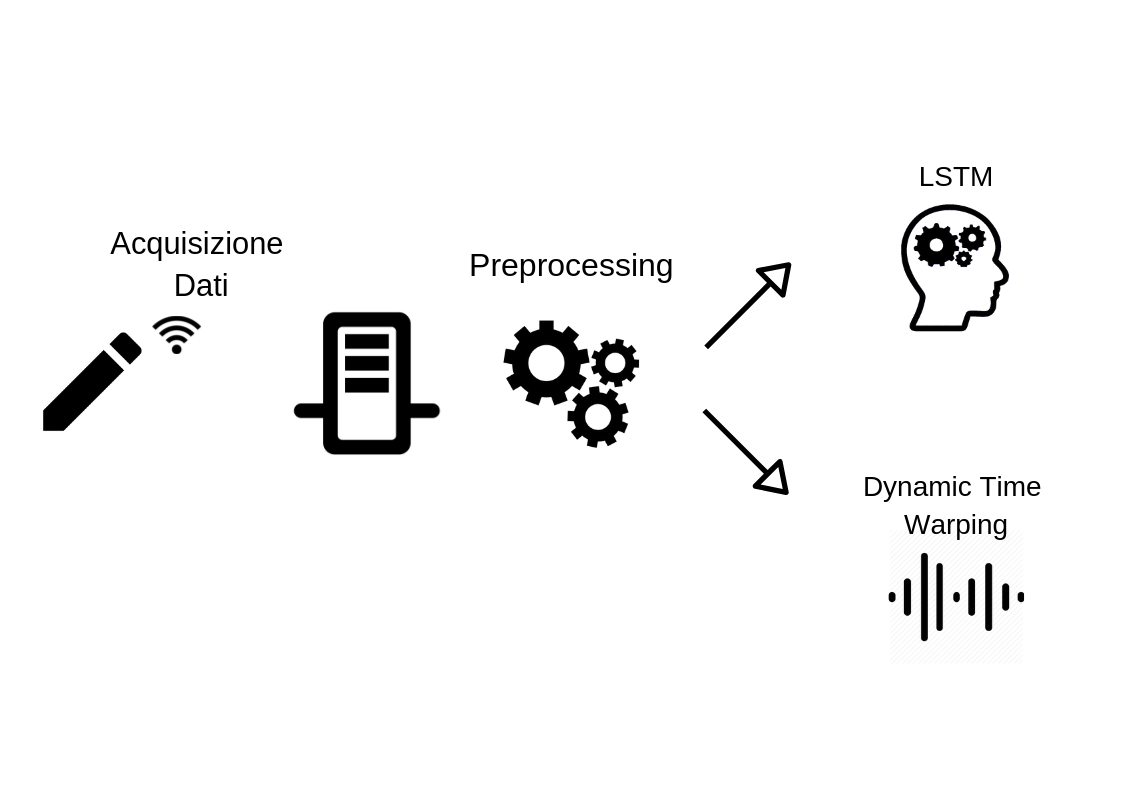
\includegraphics[scale=.25]{architettura}
			\caption{Schema dell'architettura}
		\end{center}
	\end{figure}		
	L'architettura del sistema è formata da 4 componenti: la penna, un server per l'acquisizione dei dati, e i modiuli di \textit{preprocessing} dei dati e di classificazione. La penna raccoglie i dati tramite i sensori e li invia al server attraverso il modulo Wi-Fi del chip. I dati vengono salvati in appositi file JSON sul server (ad ogni utilizzo della penna è associato un file diverso) e possono essere quindi usati dal modulo di \textit{preprocessing}. Quest'ultimo si occupa principalmente di normalizzare i dati, in modo da renderli utilizzabili dai modelli di classificazione. Un modulo di classificazione è composto da una rete neurale che utilizza delle LSTM, mentre l'altro è basato sull'algoritmo \textit{Dynamic Time Warping}.

	\section{PeterPen}
		La penna è composta dal seguente hardware:
		\begin{itemize}
			\setlength\itemsep{.1em}
			\item un chip NODE MCU ESP8266;
			\item un accelerometro;
			\item un giroscopio;
			\item un sensore di pressione;
			\item un LED verde;
			\item un condensatore;
			\item due resistenze;
			\item una batteria da 9V;
			\item un involucro realizzato in PLA.
		\end{itemize}
		L'ESP8266, il chip principale della penna, è formato da un micro-controllore e da un modulo Wi-Fi utilizzato per la comunicazione con il server. A questo sono collegati accelerometro e giroscopio (contenuti all'interno di un unico chip), il sensore di pressione e il LED. \\
		Il sensore di pressione misura la forza applicata sulla punta della penna grazie all'ausilio di una molla. Subito dopo il sensore di pressione è posizionato il chip dell'accelerometro del giroscopio e, dopo questo, si trova il microcontrollore. \\
		
		\begin{figure}[H]
			\begin{center}
				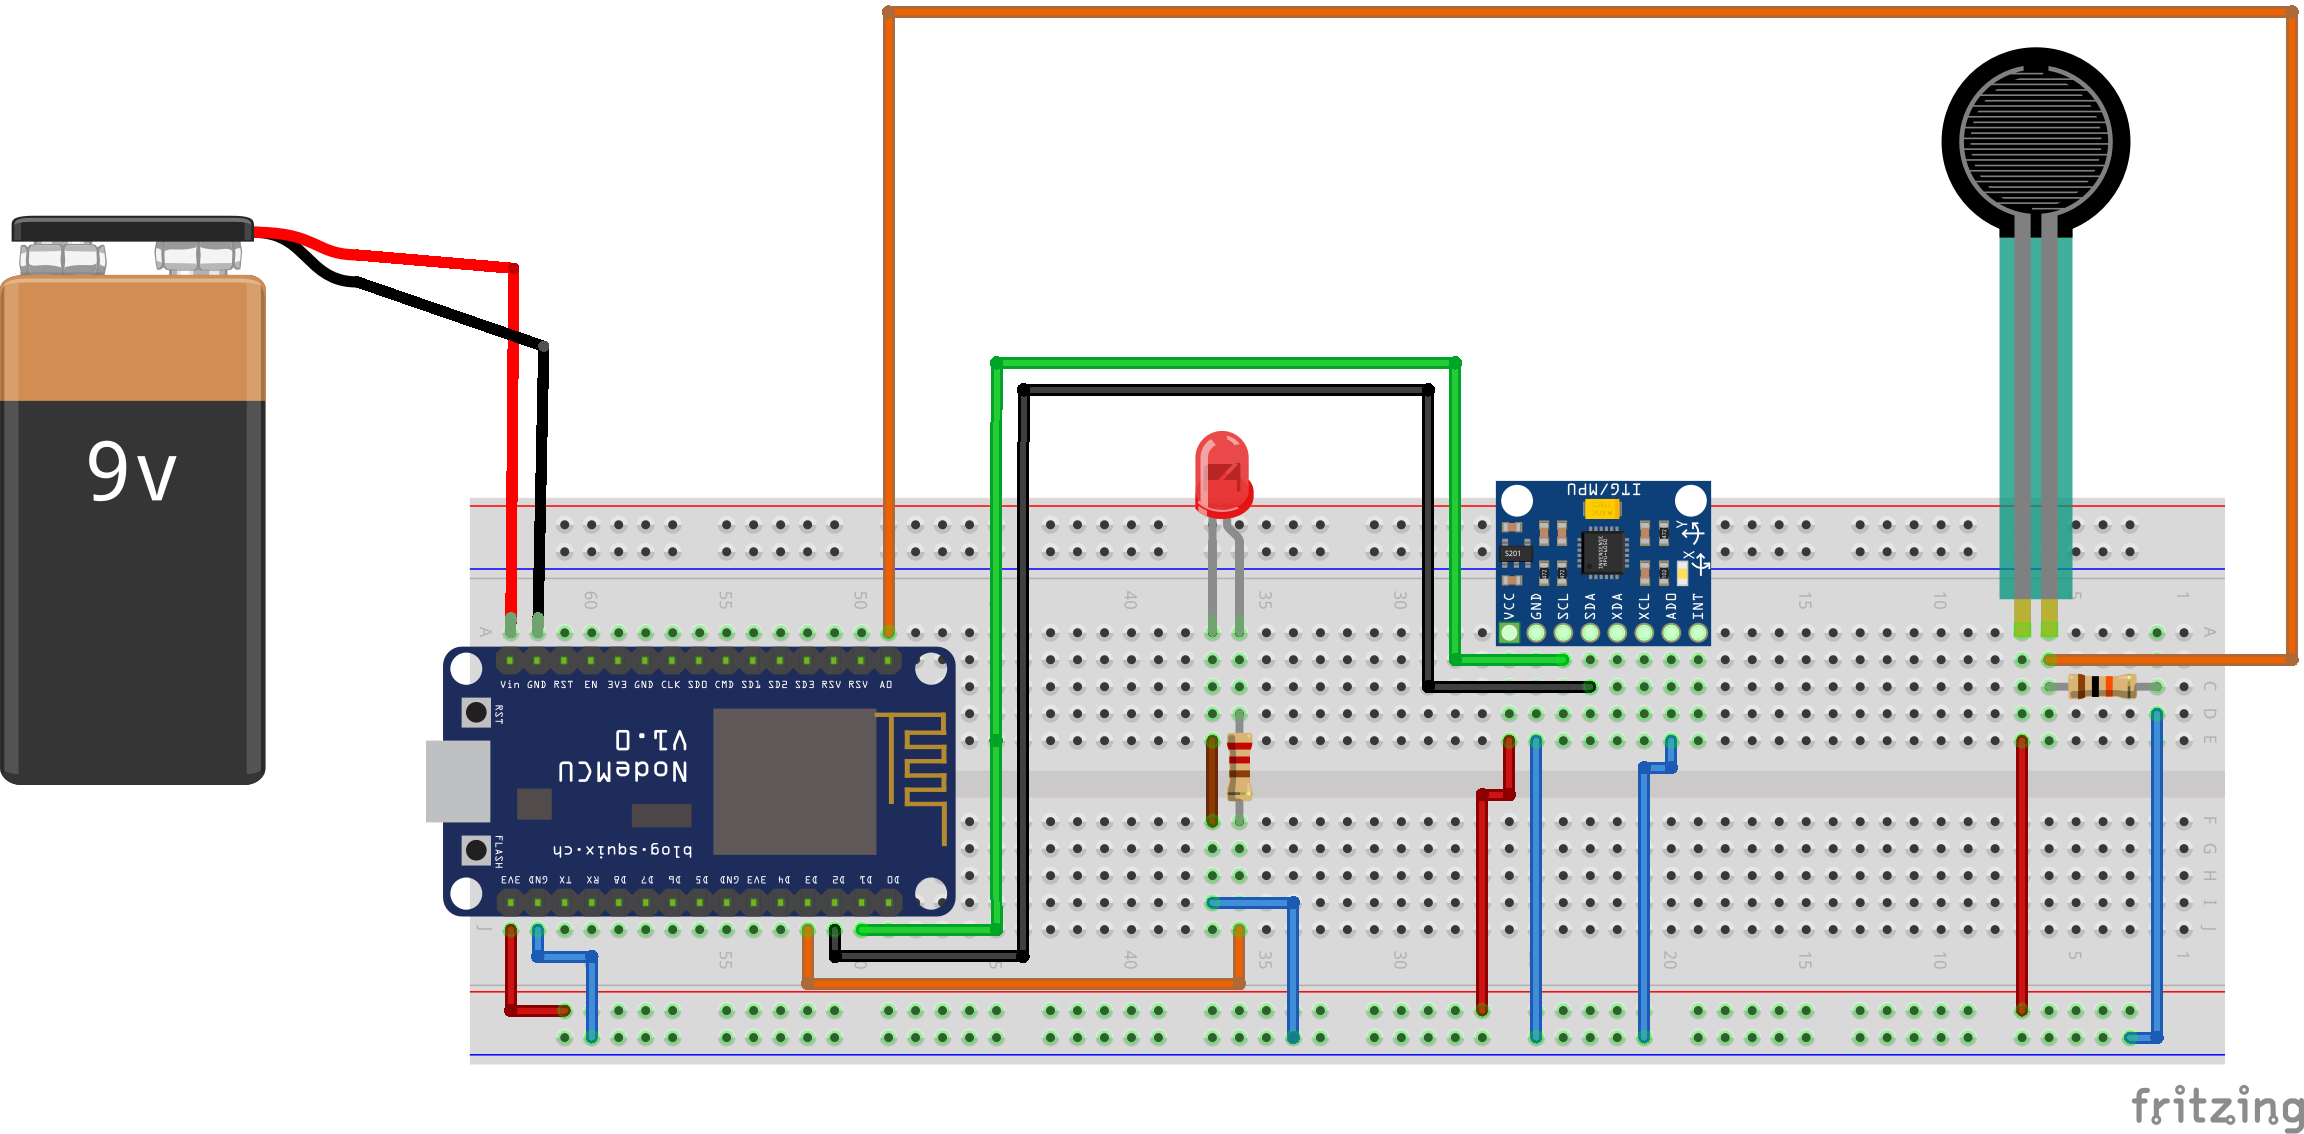
\includegraphics[scale=.35]{circuito}
				\caption{Circuito della PeterPen, realizzato con Fritzing}
			\end{center}
		\end{figure}

		\begin{figure}[H]
			\begin{center}
				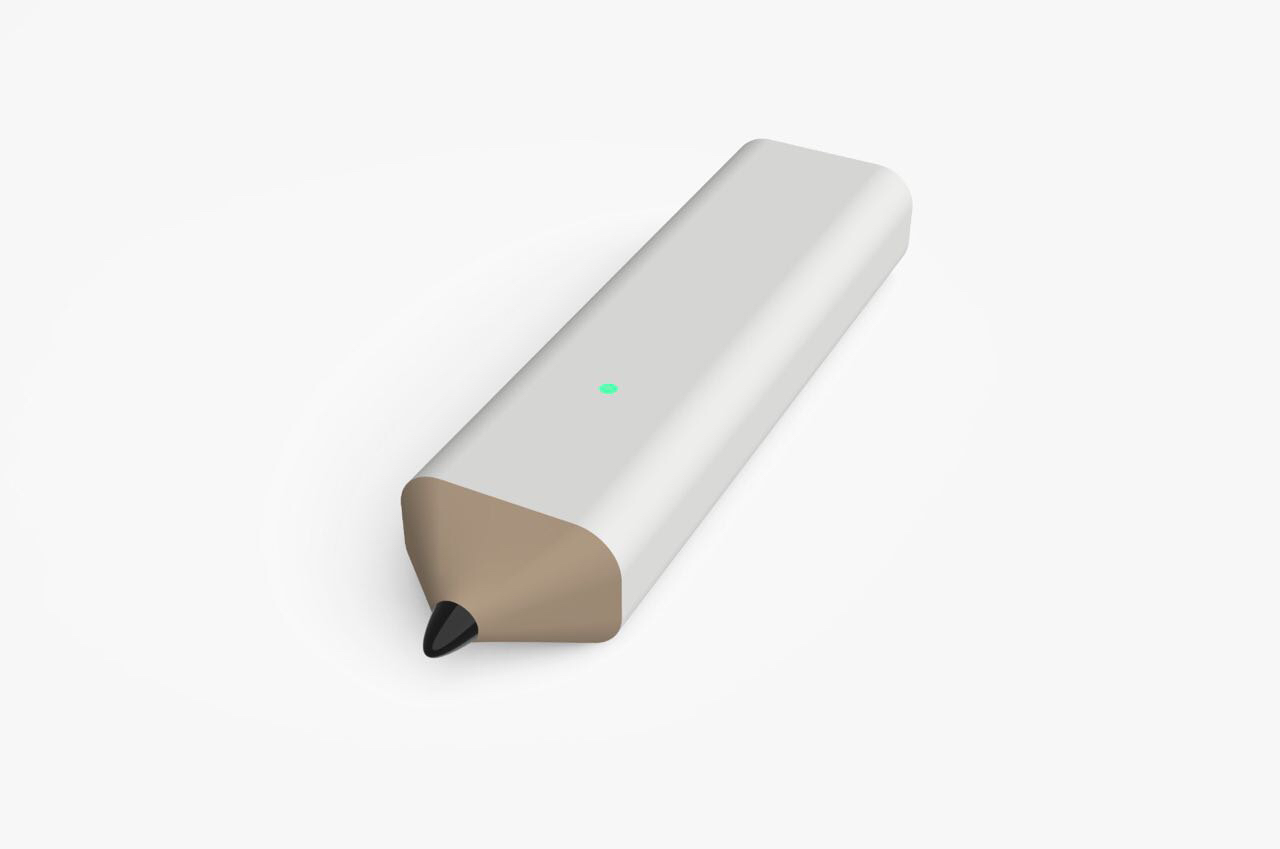
\includegraphics[scale=.1]{design}
				\caption{Design della PeterPen, si ringraziano Cristian Cianfarani e Tiziano Grossi}
			\end{center}
		\end{figure}		
		
		\begin{figure}[H]
			\begin{center}
				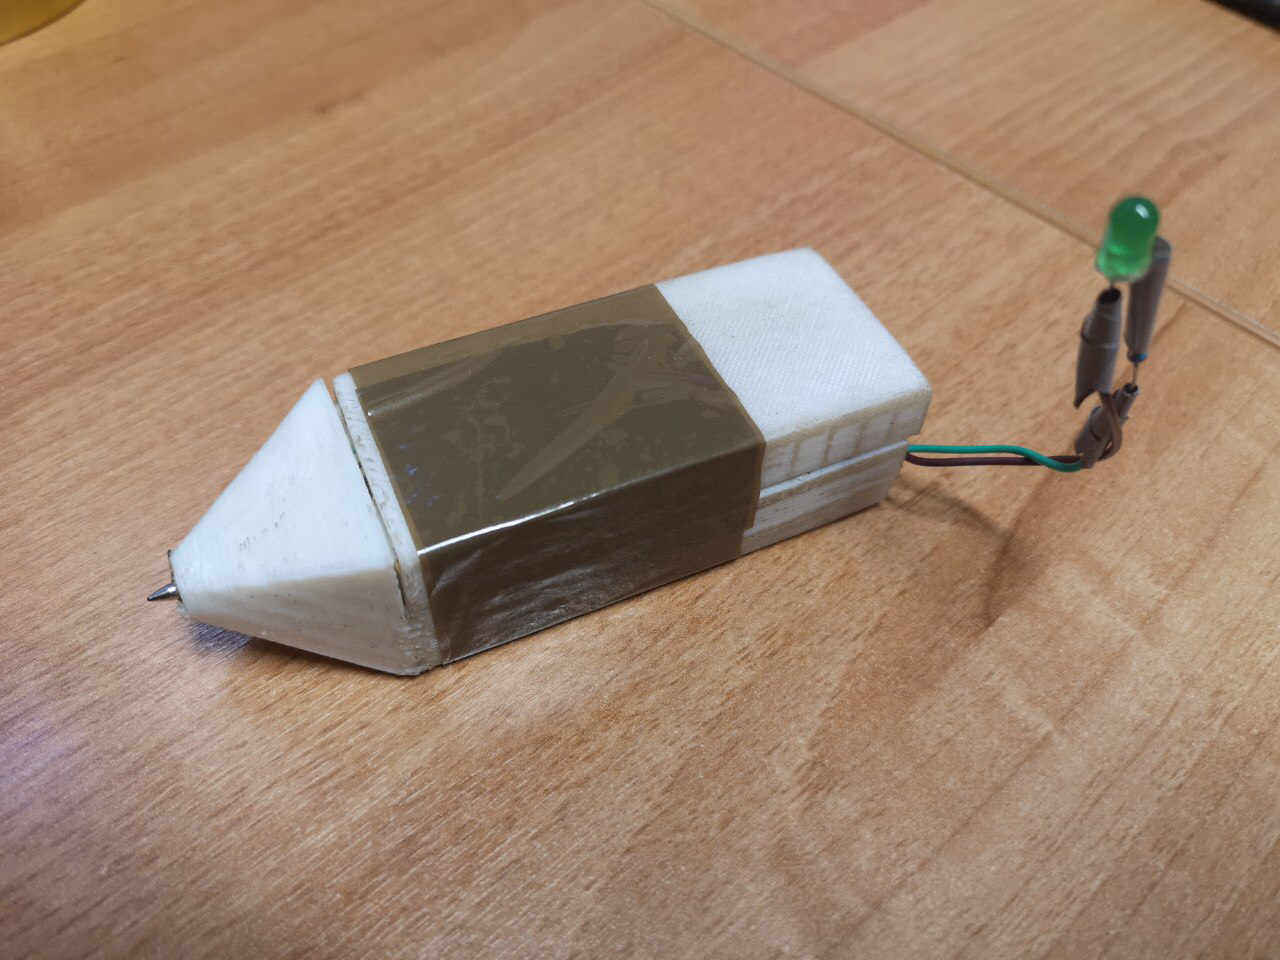
\includegraphics[scale=.1]{peterpen}
				\caption{PeterPen realizzata}
			\end{center}
		\end{figure}

		
		\subsection{Protocollo di acquisizione}
			È stato ideato un protocollo per semplificare l'acquisizione e l'invio dei dati. All'accensione della penna (o alimentandola tramite un cavo USB o tramite una batteria da 9V) il LED lampeggia durante la connessione alla rete e al server, o in caso di errore. Una volta connessa, il LED smette di lampeggiare e rimane acceso, questo indica all'utente che può iniziare a scrivere. Durante la scrittura la luce rimane spenta e, se non viene rilevata alcuna pressione per più di 2 secondi, si riaccende indicando la fine della scrittura della parola precedente e l'invio dei dati. È stato inoltre impostato come tempo massimo di scrittura 10 secondi, nel caso in cui l'utente superi tale limite il LED comincerà a lampeggiare, per segnalare l'errore e nessun dato sarà inviato.
		
		\subsection{Codice sorgente della penna}
			Il microcontrollore ESP8266 è programmato con un linguaggio derivato dal C, lo stesso che viene usato nella programmazione dei chip Arduino. Tale linguaggio richiede necessariamente l'implementazione di due funzioni in ogni programma. \\
			La prima, \verb|void setup()|, è eseguita un'unica volta all'inizio dell'esecuzione, ed è utilizzata per inizializzare le variabili. La seconda, \verb|void loop()|, rappresenta il kernel del programma ed è eseguito continuamente finché il chip è attivo, e viene eseguito ogni 10 millisecondi. \\
			Nel nostro caso, nella funzione \verb|setup|, vengono invocate altre due funzioni: \verb|mpu6050Begin| che inizializza il chip del giroscopio e dell'accelerometro e \verb|connect| che si occupa di effettuare la connessione al server. La funzione \verb|loop| ad ogni iterazione legge il valore della pressione e, in base allo stato (che è uno fra \verb|READY|, \verb|WRITING| e \verb|ERROR|) e alla variabile \verb|counter_writing| si comporterà diversamente. \\ Se la pressione registrata è sufficiente e lo stato è \verb|READY|, allora la penna passa allo stato \verb|WRITING|, acquisisce i dati e inizializza il contatore \\ \verb|counter_writing|. Invece, se la pressione è maggiore di un certo threshold, lo stato è \verb|WRITING| e sono passati meno di 10 secondi dall'inizio della scrittura allora acquisiti i dati dai sensori; nel caso in cui sono passati 10 o più secondi allora la penna si sposterà nello stato \verb|ERROR|. Infine, se lo stato è \verb|WRITING| e sono passati almeno 2 secondi da quando non si rileva abbastanza pressione, vengono inviati i dati al server e viene impostato lo stato \verb|READY|.
			
	\section{Server}
		Il server è programmato in Node.js, in ascolto sulla porta 8080 mediante una socket TCP. Ad ogni nuova connessione crea un nuovo file JSON all'interno della quale andrà a salvare tutti i dati ricevuti dalla PeterPen, effettuandone precedentemente il parsing. Nel momento in cui la sessione viene chiusa, il server si occupa di gestire la chiusura del file relativo alla stessa.
		
		\subsection{File JSON}
			Il file contiene un array di parole, ed ogni parola è composta da una sequenza di lunghezza variabile (ma lunga al più 1000) di vettori composti dalle 7 feature. \\
			Le feature raccolte sono le seguenti:
			\begin{enumerate}
				\setlength\itemsep{.1em}
				\item componenti x, y e z dell'accelerometro;
				\item componenti x, y e z del giroscopio;
				\item valore della pressione.
			\end{enumerate}
	


\chapter{Classificazione}

	\section{Preprocessing}
		Nella fase di preprocessing i dati sono stati normalizzati, effettuando uno scaling delle singole feature e aggiungendo del padding per rendere i vettori delle singole parole lunghi esattamente 1000.
	
	\section{DTW}
	
	
	\section{LSTM}
	


\chapter{Test}



\chapter{Lavori futuri}



\bibliographystyle{myIEEEtranS}
\bibliography{mybib}{}

\end{document}